\chapter{Proposta de Solução}
\label{cp:proposta}

\section{Definição dos Requisitos}

Requisito não é um termo usado apenas pela \imprimircurso. Há casos em que requisitos são apenas uma declaração abstrata em alto nível de um serviço ou restrição que um sistema deve oferecer.

\cite{sommerville} os define como: "Os requisitos de um sistema são as descrições do que o sistema deve fazer, os serviços que oferece e as restrições a seu funcionamento. Esses requisitos refletem as necessidades dos clientes para um sistema que serve a uma finalidade determinada, como controlar um dispositivo, colocar um pedido ou encontrar informações."

Na figura \ref{img:definicao_requisitos} é mostrado o processo para a definição dos requisitos. Cada atividade presente no ;processo é definido nos tópicos seguintes.


\begin{figure}[H]
	\centering
	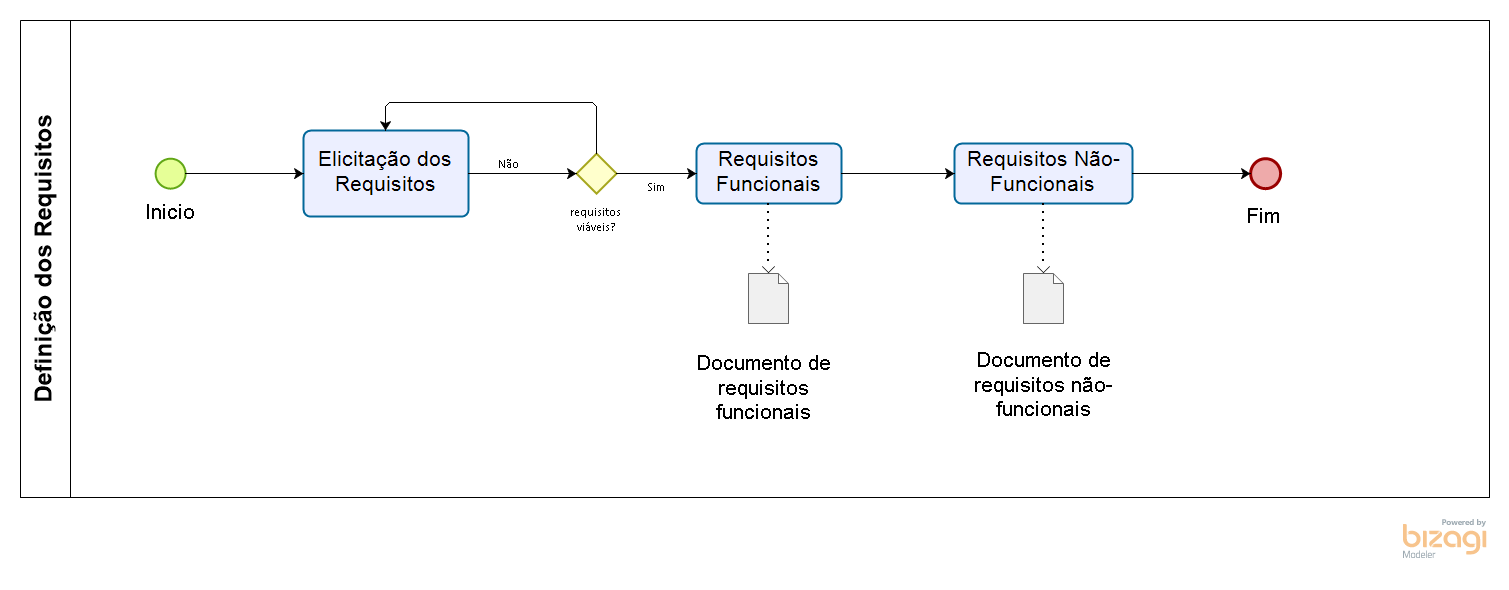
\includegraphics[width=1.0\textwidth]{figuras/elicitacaoDosRequisitos.png}
	\caption{Definição dos Requisitos. Fonte: Própria.}
	\label{img:definicao_requisitos}
\end{figure}

\subsection{Elicitação dos Requisitos}

Elicitação de requisitos é uma fase do projeto onde são extraídas informações do cliente sobre o que ele deseja que seja construído. É a fase em que o profissional de TI entende a necessidade do cliente e o orienta. É o momento de conversa com o usuário, de sentimento sobre o que este espera que seja entregue a ele. Na elicitação de requisitos são percebidas as necessidades do sistema e as características que esse sistema deve ter.

Para este projeto, foram escolhidas as seguites técnicas de elicitação de requisitos:

\begin{itemize}
    \item JAD - \textit{Joint Application Development}
    \item Entrevista
    \item Observação
\end{itemize}

\subsection{Requisitos Funcionais}
\label{sec:requisitos_funcionais}

Os requisitos funcionais descreve o que o sistema deve de fato ser. Requisitos funcionais podem ser tão específicos quanto necessário,por exemplo, podem ter sistemas com requisitos funcionais gerais e outros que além de refletir os sistemas, também abrangem as formas de trabalho de uma organização. Requisitos funcionais de um sistema deve ser completo, isso quer dizer que todos os serviços requisitados pelo usuário devem ser definidos.

\subsection{Requisitos Não-Funcionais}
\label{sec:requisitos_nao_funcionais}

Requisitos não-funcionais são requisitos que são relacionados as propriedades do sistema como confiabilidade, tempo de espera, desempenho, segurança e até restrições do sistema. Requisitos não-funcionais podem possui tanta relevância quanto os requisitos funcionais, pois em uma reunião de levantamento de requisitos, o cliente sonha o mundo e não está atento se os recursos os próprios recursos e os recursos da emprega conseguem atender ao requisito. Um requisito não-funcional não atendido pode inclusive inutilizar um projeto. Exemplo disso é caso um sistema de uma aeronave não consiga atingir a confiabilidade necessária, não será dado o certificado de segurança para operar, sendo assim a aeronave não poderá voar.